% !TEX root = ../Dokumentation.tex
\subsection{Intelligente Systeme}
\subsubsection{Softwarekonzept}
\textbf{Funktionsbeschrieb}\\[0.2cm]
Das Softwarekonzept basiert auf dem MVC\footnote{MVC = Model-View-Control} Prinzip, wobei sich die View auf einen Debug-Zweck beschränkt. Dabei hat der Controller aller Subprozesse sowie die Schnittstelle zur Harwaresteuerung, via Microcontroller-Board realisiert, unter Kontrolle. Die parallel laufenden  Subprozesse sind:
\begin{itemize}
\item Bilderzeugung
\item Objekterkennung
\item Fahrbahnerkennung
\end{itemize}
\begin{figure}[H]
	\centering
	\includegraphics[width=0.8\textwidth]{03_Loesungskonzept/pictures/grobablauf.png}
	\caption{Aktivitätendiagramm Grobablauf}
\end{figure}
Der Zustand des Fahrzeuges wird im Model gespeichert und steht allen Prozessen zu Verfügung. Die Datenstruktur ist dabei so aufgebaut, dass keine Zugriffskonflikte entstehen sollten.\\
Der Controller handelt alle Anweisungen der Prozesse. Meldet beispielsweise die Objekterkennung einen Container hat dieser Priorität vor dem normalen Fahren und das Microcontroller-Board erhält die entsprechenden Anweisungen.\\[0.2cm]
\textbf{Komponentenbeschrieb}\\[0.2cm]
Umgesetzt wird das Konzept auf dem Minicomputer in C++. Dabei werden die zuvor beschriebenen Prozesse als eigene Threads realisiert. Um eine hohe Softwarequalität sicherzustellen soll möglichst nach TDD\footnote{TDD = Test Driven Developement} gearbeitet werden. Für die automatisierten Tests werden die Open Source Pakete Google Test und Google Mock verwendet, welche in C++ realisiert und optimiert sind und sich direkt in das Projekt integrieren lassen.\\
Das Microcontroller-Board wird mit der Programmiersprache C programmiert.\\[0.2cm]
\textbf{Begründung}\\[0.2cm]
Der geplante Minicomputer verfügt über einen Vierkernprozessor, weswegen eine Parallelisierung zwingend notwendig wird, um diesen Prozessor auch vollumfänglich nutzen zu können. Bei der Programmiersprache ist C++ aufgrund der Performance und der einfachen Kopplung an C gewählt worden. Zudem sind keine Zusatztools wie virtuelle Maschinen notwendig. Die verwendete Bildverarbeitungssoftware OpenCV ist ebenfalls in C++ entwickelt und somit direkt nutzbar.\\
TDD soll sicherstellen, dass vor Allem bei kurzfristigen Änderungen keine unerwünschten Nebeneffekte entstehen und jederzeit sichergestellt ist, dass die Software wunschgemäss läuft.\\[0.2cm]
\textbf{Testergebnisse}\\[0.2cm]

\subsubsection{Mini-Computer}
\textbf{Funktionsbeschrieb}\\[0.2cm]
Der Mini-Computer beinhaltet die Logik- und Ablaubsteuerung, nimmt Bilder von der Kamera entgegen und verarbeitet diese um Container zu orten und in der Mitte der Fahrbahn zu bleiben. Die Lenkkorrektur und weitere Befehle zur Steuerung der Mechanik werden via USB Schnittstelle an as Mikrocontroller-Board weitergeleitet.\\[0.2cm]
\textbf{Komponentenbeschrieb}\\[0.2cm]
\begin{figure}[H]
	\centering
	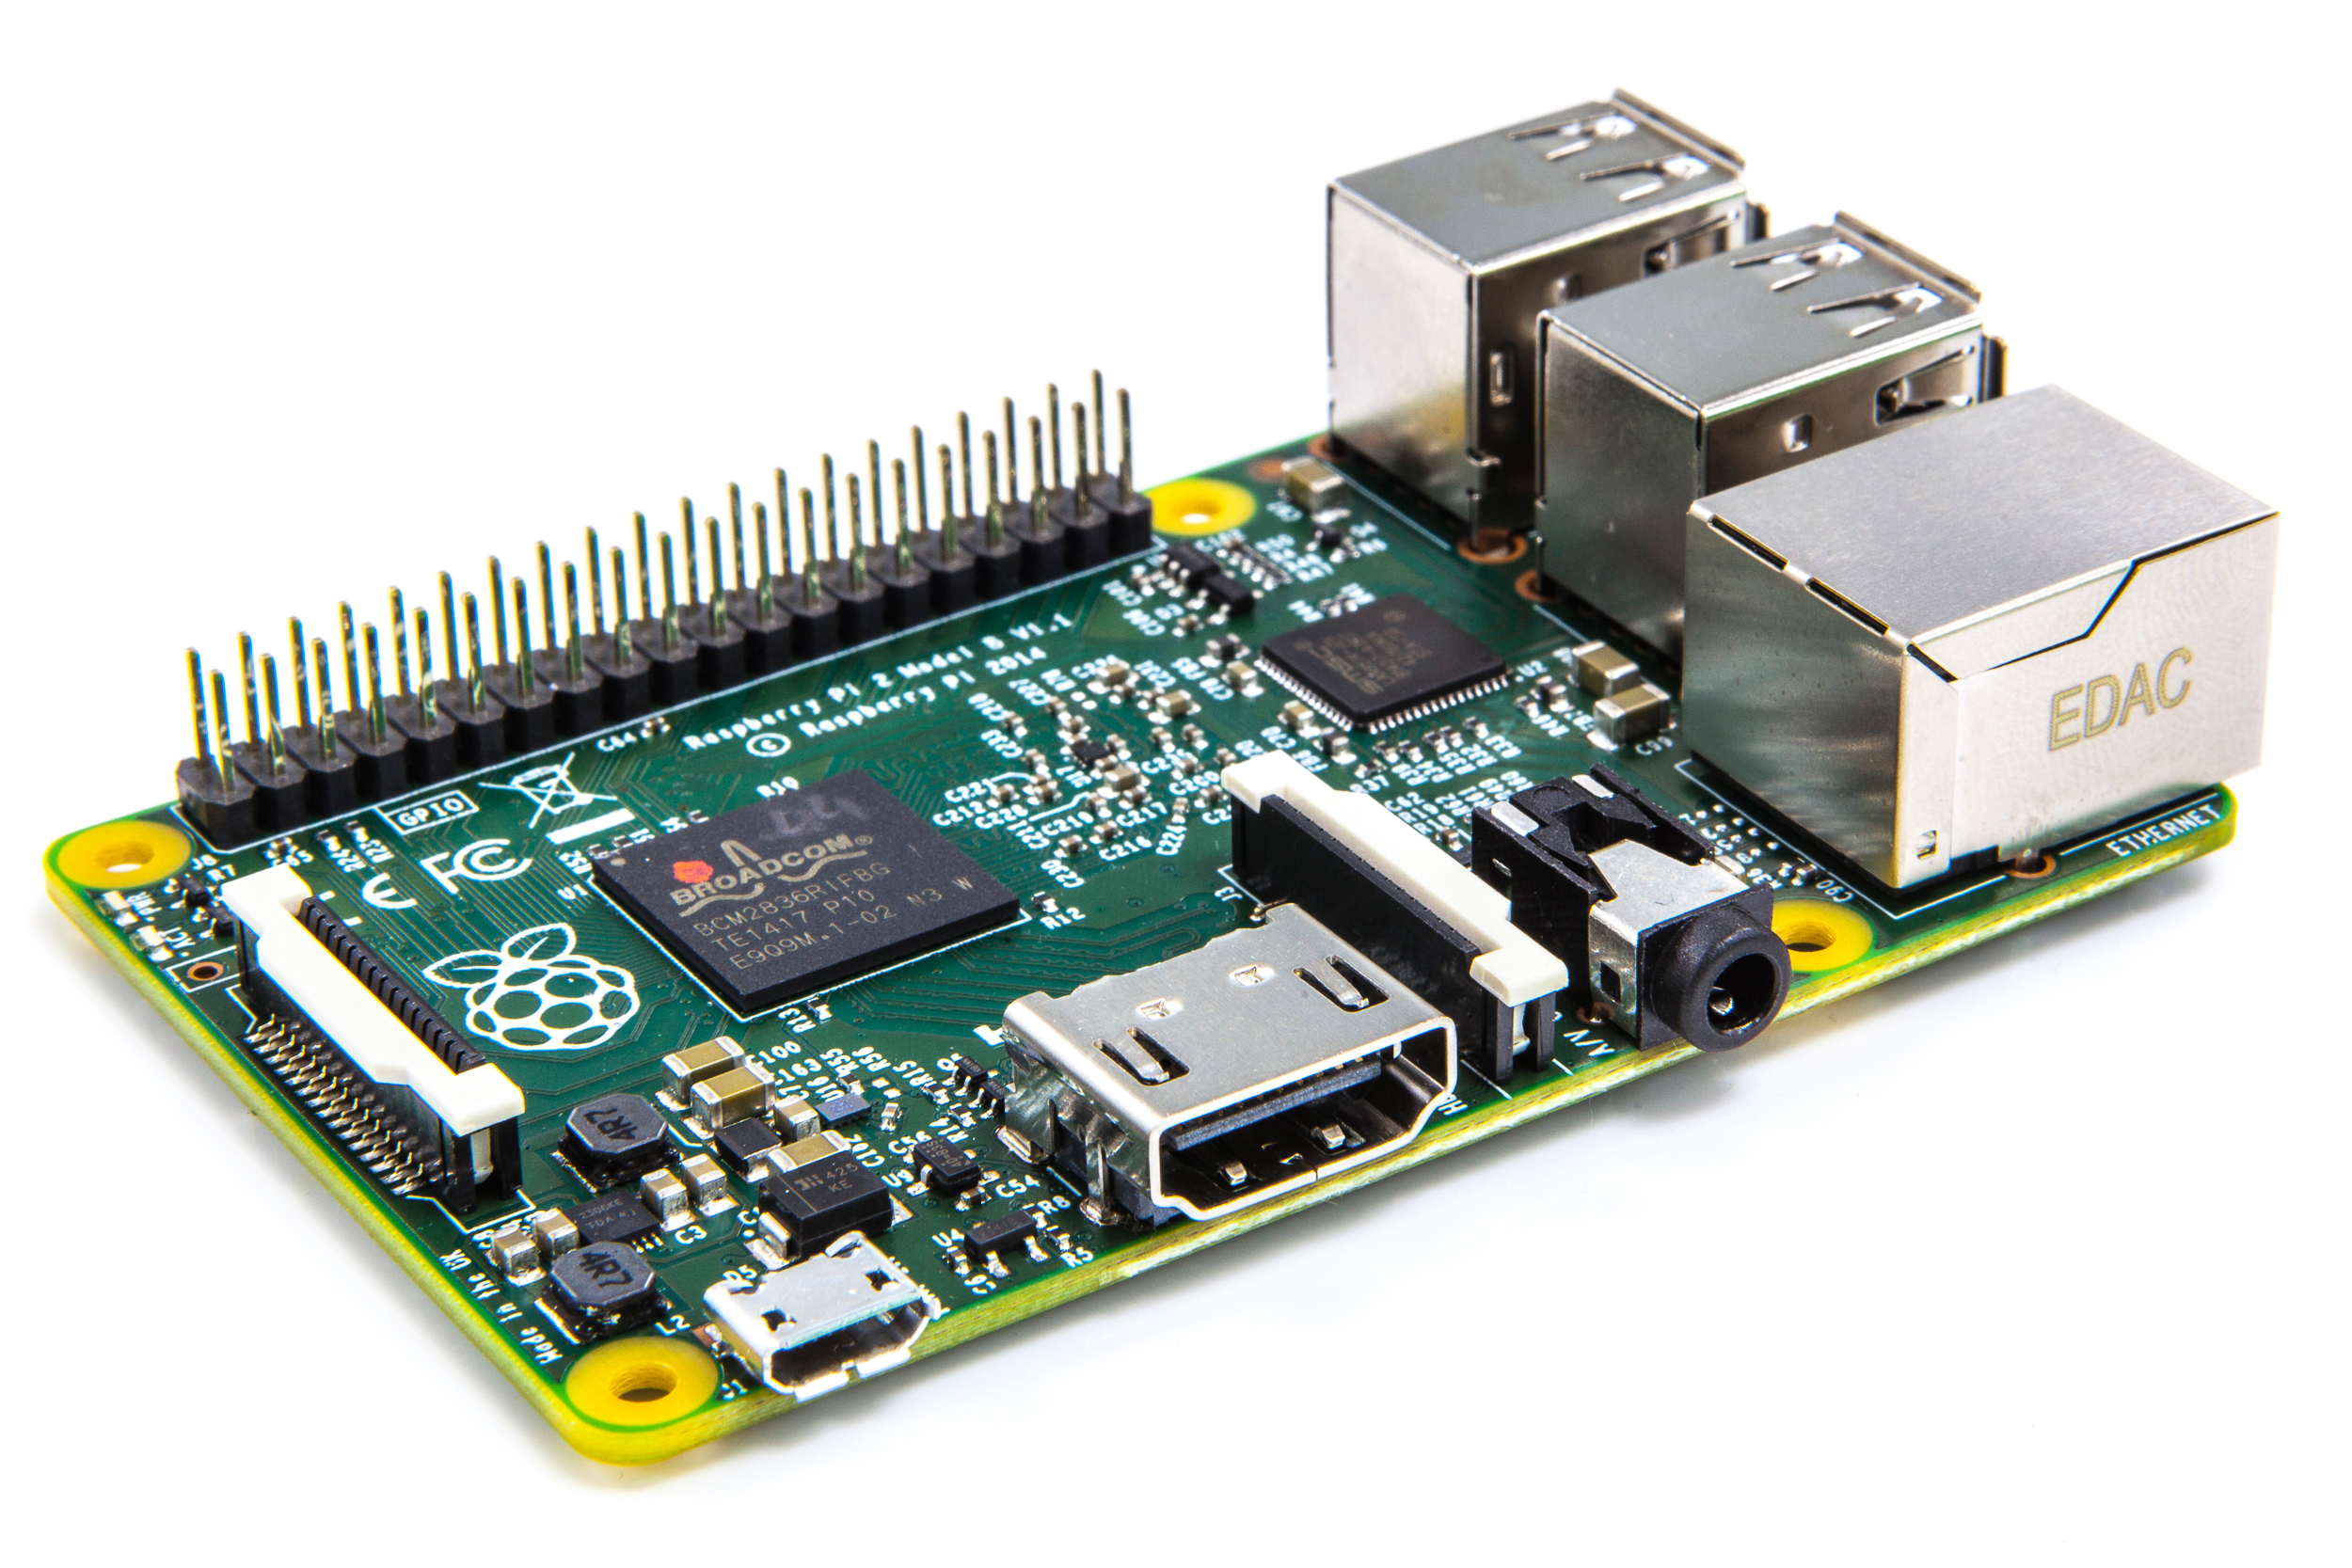
\includegraphics[width=0.5\textwidth]{03_Loesungskonzept/pictures/raspberrypi2.png}
	\caption{Raspberry Pi2 Model B (Quelle:http://pcworld.com/)}
\end{figure}
Das Raspberry Pi2 bietet mit einem 900MHz Quadcore Prozessor, einem eigenem Grafikchip und 1GB Ram viel Leistung und ist ideal geeignet.\\[0.2cm]
\textbf{Begründung}\\[0.2cm]
Dem Team war von Anfang an klar, dass die Bildverarbeitung viel Ressourcen verbrauchen wird. Gleichzeitig darf der Energieverbrauch die Kapazität eines Akkus nicht übersteigen. Das Raspberry Pi2 besitzt genügend Leistung und ist trotzdem sparsam. Mit einem Quadcore und 1GB RAM ist es ausreichend performant um Bilder zeitig zu verarbeiten. Zusätzlich ist es einfach zu verwalten und bedienen, da es ein eigenes Betriebssystem besitzt.\\[0.2cm]

\subsubsection{Mikrocontroller-Board}
\textbf{Funktionsbeschrieb}
Das Mikrocontrollerboard bildet die Schnittstelle zwischen der Hardware (Motor, Sensoren, Servos..) und dem Minicomputer. Das Mikrocontrollerboard übernimmt die Ansteuerung und Auswertung der einzelnen Komponenten und stellt die verarbeiteten Informationen dem Minicomputer über eine Schnittstelle zur Verfügung. \\[0.2cm]
\textbf{Komponentenbeschrieb}\\[0.2cm]
\begin{figure}[h]
	\centering
	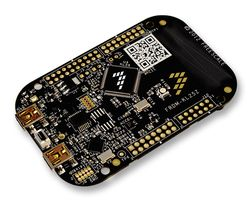
\includegraphics[width=0.5\textwidth]{03_Loesungskonzept/pictures/freedomboard.png}
	\caption{Freedomboard KL25 von Freescale (Quelle:http://ch.farnell.com/)}
	%http://ch.farnell.com/productimages/standard/de_DE/freescalesemiconductor-frdm-kl25z-40.jpg
\end{figure}
Als Mikrocontrollersystem wurde das Freedomboard KL25Z von Freescale ausgewählt. Das Entwicklungsgsboard bietet vieles, wie ausreichend I/O's, AD Wandler und Timerausgänge. Das Bord wird mit der Programmiersprache C programmiert. \\[0.2cm]
\textbf{Begründung}
Das Board überzeugt durch eine gute Rechenperformance zu einem kleinen Preis. Das Hauptargument für das Freedomboard ist die einfache Programmierung. Für viele Komponenten wie Servos oder Ultraschalsensoren steht ein Tool namens ProcessorExpert zu Verfügung. Diese Tool ermöglicht eine relativ einfache Anbindung solcher Komponenten. Dies spart sehr viel Entwicklungsaufwand.
Das Freedomboard hat sich gegen das Tinkerfogesystem durchgesetzt. Der Hauptgrund ist Flexibilität des Freedomboard gegenüber dem Tinkerfogesysem. Das Tinkerforgesystem ist sehr einfach zu bedienen solange alle Komponenten von Tinkerfogre zu Verfügung gestellt werden. Fehlt aber ein Modul wird es sehr schnell kompliziert. Beim Freedomboard ist der Aufwand für eine Komponente etwas höher, dafür können die meisten Systeme angeschlossen werden.\\[0.2cm]
\textbf{Testergebnisse}
Das Freedomboard wurde als Funktionsmuster bereits in Betrieb genommen. Es hat sich gezeigt, dass die Anbindung der Komponenten Tatsächlich sehr einfach ist. Es wurden bereits ein Ultraschallsensor, mehrere Servos, eine UART Kommunikation und ein Infrarotsensor angebunden. Das System sah dabei sehr vielversprechend aus.\\[0.2cm]
\textbf{Software Grundaufbau}\\[0.2cm]
Das Tool ProcessorExpert bietet eine Komponente FreeRTOS an. Das ist ein Betriebssystem, welches das Programmieren sehr vereinfacht. Damit können verschiedene Tasks definiert werden und quasi parallel ausgeführt werden. Die Software wird damit geplant. Folgende Tasks sind geplant.
\begin{figure}[h]
	\centering
	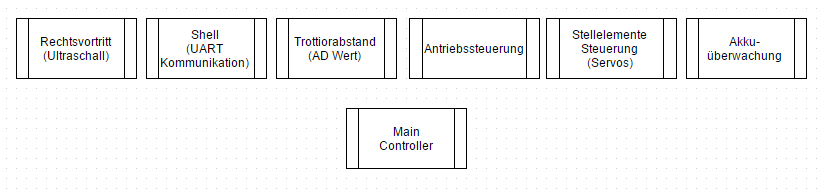
\includegraphics[width=0.9\textwidth]{03_Loesungskonzept/pictures/MC_Tasks.png}
	\caption{Übersicht MC Tasks}
\end{figure}
Die Implementierung der Task wird im PREN2 eingegangen.